\section{Durchführung}
\label{sec:Durchführung}
%wär cool wenn du schreibst, wo wir die Gewichte aufgehangen haben.
Zu Beginn werden die verwendeten Stäbe ausgemessen. Hierbei wird die Länge, der
Durchmesser sowie das Gewicht notiert.
In folgender Abbildung \ref{fig:aufbau} ist der Aufbau des Versuches schematisch dargestellt.
\begin{figure}[H]
  \centering
  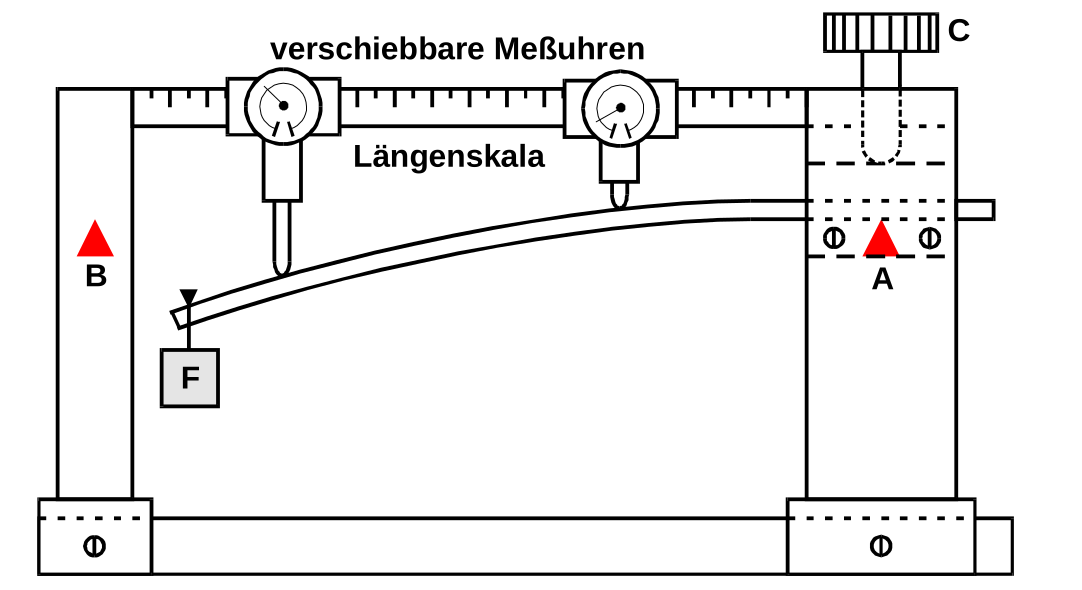
\includegraphics[scale=0.4]{content/versuchsaufbau.png}
  \caption{Schematischer Aufbau der verwendeten Apparatur.}
  \label{fig:aufbau}
\end{figure}
Hierbei können die Probenstäbe entweder einseitig oder beidseitig eingespannt
werden. Die Gewichte werden bei einseitiger Einspannung 
